% 1977 年上海卷理科附加题：半圆与等边三角形
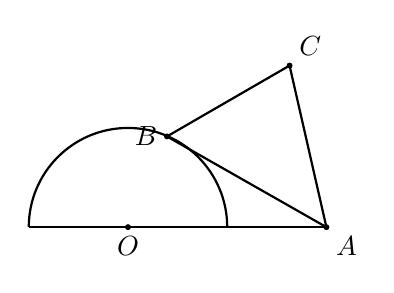
\begin{tikzpicture}[scale=0.9]
  \coordinate (O) at (0,0);
  \coordinate (L) at (-1.4,0);
  \coordinate (R) at (1.4,0);
  \coordinate (A) at (2.8,0);
  \coordinate (B) at (0.55,1.28);
  \coordinate (C) at (2.28,2.28);
  \draw[thick] (L) arc (180:0:1.4);
  \draw[thick] (L)--(A);
  \draw[thick] (B)--(A)--(C)--cycle;
  \fill (O) circle (1.2pt) node[below] {$O$};
  \fill (A) circle (1.2pt) node[below right] {$A$};
  \fill (B) circle (1.2pt) node[left] {$B$};
  \fill (C) circle (1.2pt) node[above right] {$C$};
  \draw[dashed] (O)--(A);
\end{tikzpicture}
